% Drawing 156-2/01-1 -- folder 156-2, batch 01, archive page 12 (PDF page 13).
% Transcription: en marge, un croquis : une bande allongée, $A$ à gauche, deux traits transverses $C$ et $D$, $B$ à droite
% Kind: elongated strip with transverse strokes. Method 2 (schematic redraw from the facsimile). Status: ok.
% Notes: A long strip, its left end a thick stroke A, two transverse thick strokes C and D, open at the right end B. The long diagonal line crossing the sketch is one of the strokes striking the page and is not drawn.
% Coordinates: 1 unit = 1 mm = 1/100 of the crop width (bbox in page fractions: [0.07, 0.43, 0.35, 0.53]).
% Redrawn by Claude (claude-opus-5-5), issue #73, 2026-11-07; not checked by a human; not compiled (no TeX in the session).
% Rights: reproduces part of the work -- behind RENDER_TRANSCRIPTS, never published by itself.
\documentclass[tikz,border=3pt]{standalone}
\usepackage{amsmath,amssymb}
\usetikzlibrary{patterns,arrows.meta}
\tikzset{pencil/.style={black!45}, struck/.style={black!35}, mark/.style={circle,draw,inner sep=1.3pt}, pt/.style={circle,fill,inner sep=0.9pt}, opt/.style={circle,draw,fill=white,inner sep=1.1pt}}
\begin{document}
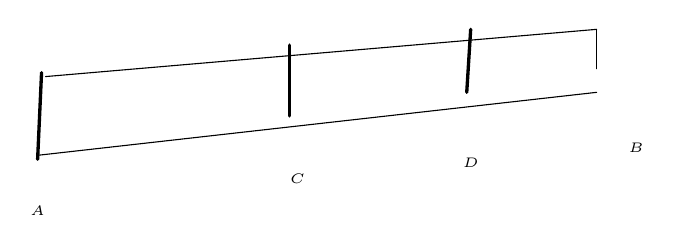
\begin{tikzpicture}[x=1mm,y=1mm,line cap=round,line join=round,font=\scriptsize]
\draw (23,-25) -- (93,-19);
\draw (22,-35) -- (93,-27);
\draw[very thick] (22.5,-24.5) -- (22,-35.5);
\draw[very thick] (54,-21) -- (54,-30);
\draw[very thick] (77,-19) -- (76.5,-27);
\draw (93,-19) -- (93,-24);
\node[inner sep=1pt] at (22,-42) {\tiny $A$};
\node[inner sep=1pt] at (55,-38) {\tiny $C$};
\node[inner sep=1pt] at (77,-36) {\tiny $D$};
\node[inner sep=1pt] at (98,-34) {\tiny $B$};
\end{tikzpicture}
\end{document}
